\section{Mathematical Modeling}
\label{sec:mathmodel}

% \begin{itemize}
% \item \st{unstable stratified boundary layers (raleigh number estimate)}
% \item \st{justify incompressible N-S}
% \item \st{justification of far-field eddy-viscosity model (M-O)}
% \item modeling eddy-viscosity in device 
% \item vane and turbine representation via penalty function // immersed boundary method
% \item cone representation
% \end{itemize}

%remember that \st{} is strikethrough
%
% should this all be math modeling?
%

The aim of the proposed work is to simulate the formation of synthetic
dust devils in the field. This requires a model of the ambient conditions for a
representative case, such as Arizona, where experimental data is
available from test that have been performed. Furthermore, for this to be
more generally useful in the prediction of flows in a variety of
conditions, we need a model generally applicable to any flow near the
surface of the earth.  

This section details an analysis of surface fluid mechanics, and
develops a mathematical model for turbulence in a thermally stratified
medium. We seek to emulate the operation of the apparatus during the day, 
when dust devils are observed to form readily. 
At these times, the atmospheric surface layer has the following character. 
Incident radiation from the sun does not significantly interact with the
air, which is nearly transparent. Instead, this radiation is absorbed by
the ground, which causes it's temperature to rise. This results in a thermal
gradient between the hot ground and the cooler air. The warm ground
conducts heat to the air, causing expansion and lowering the density
of the air. This reduced density air near the surface is driven upwards
by the force of buoyancy.  

For sufficiently large temperature gradients, these motions are
unstable, and as the warm air is driven upwards the flow will transition
to turbulence. For the typical use case we consider, namely Arizona in
summer, the temperature difference can be in excess of 30 Kelvin. 
Rayleigh numbers associated with temperature gradients of this magnitude
this are between $10^{9} - 10^{11}$, and therefore meet the criterion
for transition to a turbulent regime. The flow is that of an unstably
stratified fluid.  

This section begins with\todo{write me!}

Note that a complete mathematical specification of all the model
parameters introduced in this section are provided in a table in
appendix \ref{app:model_param}.

\subsection{Equations of Fluid Motion}
%
% do I need to justify this more? These are pretty critical, after all
%

The equations describing fluid flow at
low Mach number with natural convection are, %\todo{fix me up}
\begin{eqnarray*}
 \frac{\partial u}{\partial t} + u \cdot \nabla u =&
  -\frac{1}{\rho}\nabla P + \nu \nabla^2 u - g \frac{T'}{T_0}\\
 \nabla \cdot u =& 0 \\
 \rho c_p \frac{\partial T}{\partial t} + u \cdot \nabla T =& \nabla \cdot ( k \nabla T).
\end{eqnarray*} 

Where we have made the assumptions that the temperature variation is small in
comparison to the mean temperature of the region. These are the
incompressible Navier-Stokes equations with Boussinesq representation of
buoyancy coupled with the heat equation.  
%
% in full document be sure to mention that neglecting coriolis is legit
% below 50ms
%
%
As discussed above, we anticipate our flow to be
turbulent. Turbulence significantly alters the character of the flow,
and necessitates either resolving the resulting small scales or
providing a model that emulates their impact. In this case, we use a
Reynolds Averaged Navier-Stokes (RANS) formulation, where we 
permit the viscosity and thermal conductivities to vary in space, and
decompose the flow into constant laminar and varying turbulent and vane
components,  

% \begin{eqnarray*}
%  \nu =& \nu_{l} + \nu_{T}(z) + \nu_{V}(r,z) \\
%  K =& K_{l} + K_{T}(z) + K_{V}(r,z)
% \end{eqnarray*}

\begin{eqnarray*}
 \nu =& \nu_{l} + \nu_{T}(z) + \nu_{V}(r,z) \\
 K =& K_{l} + K_{T}(z) + K_{V}(r,z).
\end{eqnarray*}

This is an effective eddy viscosity model, and the subsequent two
sections will elaborate on the spatial dependence and character of
$\nu_T$, $K_T$, $\nu_C$ and $K_C$. $\nu_l$ and $K_l$ are the laminar,
base diffusivities and do not vary in space. 

\subsection{Viscosity Model}

We use the celebrated similarity model of Monin and
Obukhov\cite{monin2007statistical,monin1954basic} as a guide to the
present development, which we outline below. Their formulation is an
extension of the mixing-length model of Prandtl, where the concepts of
gradient diffusion and mixing length were generalized to thermally
stratified flow.   

%
% justify prandtl assumption here
%

Under temporally steady, horizontally homogeneous conditions, the 
dynamics of any mean turbulent quantity ($\bar f$) in a 
thermally stratified medium which depends only on,  

\begin{equation}
\bar f = f(z,\frac{g}{T_0},\rho_0,\nu_l,K_l,u^*,q).
\end{equation}

These five parameters are: the distance from the ground, z; the
buoyancy coefficient, $\frac{g}{T_0}$; the density of the fluid,
$\rho_0$; a velocity scale, $u^*$; and the heat flux from the ground,
$q$. 


% Aside from near the surface, the diffusivities $\nu_l$ and $K_l$ will be
% small compared to their turbulent counter-parts, $\nu_T$ and $K_T$. 
% Likewise, if we define $z-z_0$ as an ``effective roughness
% height'' or displacement distance, we can reasonably neglect $z_0$ from these
% considerations. While the roughness height can be large (for instance in
% a cornfield, where the roughness height could reasonably be several
% meters), for the present study the expectation is that this roughness
% height will be on the order of centimeters\cite{oke1987boundary}, and
% therefore negligible.  
%
% add refence to dynamical and physical meteorology 
% 
These quantities depend on four dimensions: length, time, temperature
and mass. Dimensional analysis implies that this mean turbulent quantity
($\bar f$) should then only be a function of a single dimensionless
group.\cite{munson2012fundamentals}. This is chosen to be,
\begin{equation}
 \xi = \frac{z}{L}.
\end{equation}
Here, $L$ is the famous, ``Monin-Obukhov'' length,
\begin{equation}
 L = -\frac{{u^*}^3}{\kappa \frac{g}{T_0} \frac{q}{c_p \rho_0}}
\end{equation}
where $\kappa$ is the (dimensionless) Von-Karman constant. Notice that
our interest lies in regimes where $L<0$, as $q<0$ (e.g. heat from the
ground into the fluid), which corresponds to the unstable stratification 
we expect during a sunny day. The mean quantity $\bar f$ has a
functional representation to the effect,
\begin{equation}
 \bar f = C \phi(\xi)
\end{equation}
with C a multiplicative constant with units of $\bar f$, and $\phi$ is a
function only of $\xi$. We are interested in the case where $\xi<0$, which
corresponds to heat flux from the ground into the air.\todo{clean the
rest of this up}

The case where $\xi \to -\infty $ implies $\frac{z}{L} \to
-\infty $ and $z>>L$. This is most readily interpreted as the instance
where $u^* \to 0$, e.g. the buoyancy-dominated case with no wind. For
this case, the function $\varphi_T$ must hold no dependence on $u^*$,
and will approach a constant value. Scaling analysis implies that the
overall function will not depend on $u^*$ only when the function
$\varphi$ scales to the $-\frac{4}{3}$ power. The resulting function
appears as

\begin{equation}
 K_T = \frac{1}{C_T} \left( \frac{q}{c_p \rho_0} \frac{g}{T_0}
		     \right)^\frac{1}{3} z^{\frac{4}{3}}  \text{ 
for } z \gg L. 
\end{equation}

So long as the Prandtl number remains constant in space, then
% todo: provide discussion as to why this is not an unreasonable expectation
identical arguments as to the asymptotic behaviour at large $\xi$ provide
the analogous result for the eddy viscosity's variation with respect to
distance from the ground,  
\begin{equation}
 \nu_T = \frac{1}{C_{\nu_T}} \left( \frac{q}{c_p \rho_0} \frac{g}{T_0}
			     \right)^\frac{1}{3} z^{\frac{4}{3}}  \text{ 
for } z \gg L. 
\end{equation}

These functions have been found to be broadly applicable and
accurate\cite{Foken2006}, and are easily instantiated in software.

\subsection{Eddy Viscosity in Device}

%However, this is also a more
%difficult regime to model.\todo{poor justification} 
The validation process identified a refinement to the virtual vane
formulation that results in a better representation of the vane
effects in a broader range of flows. 

The thermal and momentum diffusivities are even larger in the
device where the flow across the vanes produces shear and generates
turbulence. The model now include an enhanced turbulent diffusivity in
the vortical plume region to account for the effects of vortex shedding
from the trailing edge of the vanes, which is not inherent in the
virtual vane representation.   

% To successfully accomplish this, source terms
% for production of diffusivity were formulated to properly
% account for the generation of turbulence in the region of the
% vanes. This diffusivity would then convect and diffuse through space. 
% To avoid modeling a temporal and three-dimensionally spatially
% varying field of diffusivities, we have instead calibrated the field
% based on data provided by our partners at Georgia Tech. 

%This calibration
%is detailed in Section \ref{sec:validation}. 
The eddy-viscosity in the region of the vanes and interior is set based
on scaling relations for a turbulent self-similar circular jet, as in 
Pope\cite{pope2000turbulent}
 
\begin{equation}
  \nu_C = U_0 y_{1/2} \bar \nu_C.
  %\nu_C(r) = U_0(r) y_{1/2}(r) \bar \nu_C
\end{equation}

In this equation, $U_0$ is the peak velocity, and $y_{1/2}$ the jet
half-width (taken to be the dust devil half-width).  
% In words, we are scaling the
% calibrated viscosity by the velocity and length scale of the
% apparatus. $\bar \nu_C $ is input, measured from the experimental
% laboratory.  The diffusivity here is essentially a top hat filter, which
% radial values interior to the vanes the nominal calibrated value, and
% those outside the vanes zero, e.g. $\nu_C(r>r_{\text{vane}})=0$. 
The dimensionless constant $\bar \nu_C $ is calibrated based on
experimental data, and is set to zero outside the device. 
The thermal diffusivity inside the device, $K_C$, is then fixed with the 
assumption that the Prandtl number is unity.  

%The thermal and momentum diffusivities are expected to be even larger in the
%device where the flow across the vanes produces shear and generates
%turbulence. Our model for the diffusivities inside the vanes should
%therefore be higher than the ambient regions outside the vanes. 



\subsection{Vane and Turbine Representation}
\label{subsec:vane}
To rapidly prototype general system configurations, the
computations must be able to explore a large space of possible
geometries and settings. This presents a significant meshing and 
computational challenge if the detailed flow around the vanes is to be
computed. In the region near the vanes, where a no-slip boundary
condition is imposed, the flow will necessarily form a thin momentum
boundary layer. Resolving this boundary layer requires high resolutions
immediately adjacent to the walls. Changing the vane location requires
that a new mesh be generated.
This is a significant
challenge, as the development of a new mesh often requires significant
human effort and time. Furthermore, the process is error-prone, 
and would require that each simulation using a new mesh undergo 
detailed solution verification. 


% Your text on the virtual vanes does not provide enough information to
% know exactly what we did. It is needlessly vague, and does not
% adequately connect to the real vane geometry. I propose the following
% more direct and more precise text. Further, the penalty nomenclature
% is inappropriate.

Instead, we have developed a modeling formulation that does not require
explicitly meshing the turning vanes, or any surface. These so-called
"virtual vanes" are implemented as a body force that 
is applied in the annular region that contains the vanes. Vane
geometry is specified by the angle $\phi$ a vane makes with a radial
line as a function of the radial coordinate $r$. A unit normal to vane
surfaces ${\bf n}$ is thus defined as
%
\begin{equation}
 {\bf n}({\bf x}) = \sin \left(\phi(r) \right) \hat{{\bf r}}+ \cos \left(\phi(r) \right) \hat{{\bf \theta}}
\end{equation}
%
where $\hat{{\bf r}}$ and $\hat{{\bf \theta}}$ are unit
vectors in the radial and azimuthal directions respectively.
With this vane-normal vector field specified, a body force ${\bf f_v}$
is defined
that will drive the velocity in the ${\bf n}$ direction toward zero,
effectively turning the flow to be parallel to the vanes. The body
force is defined:
\begin{equation}
 {\bf f}_v= -\frac{1}{\ell_v}|{\bf u}|({\bf u}\cdot{\bf n}){\bf n}
 \label{eqn:body_force}
\end{equation}
with ${\bf u}$ the velocity and $\ell_v$ is a specified length
scale. The length scale $\ell_v$ represents the distance over which the
flow must evolve under the influence of the body force before the
velocity in the normal direction is reduced by a factor of $1/{\bf
e}$. It is a modeling constant and is specified to be of order the
separation distance between neighboring vanes in the physical vane
configuration, since entry lengths in internal flows scale with the
size of the channel.

This virtual vane formulation is similar to the actuator disk model
commonly used to represent the rotor of a wind turbine \cite{betz}.


\subsection{Solid Surface Representation}
\label{subsec:solid_surface}

This subsection details the model used for rigid, impermiable surfaces
such as the wind break (``cone'') on the top of the facility. As with
the turning vanes, this is accomplished without explicitly meshing the
surface nor imposing  a boundary condition at the surface. This permits
rapid exploration of configurations  with different solid surfaces to
control and manipulate the fluid flow. These solid surfaces are also
represented by a body force region applied where the wall is set to be
located in.  A vector normal to the surface is defined in this region so
that a body force will push  the velocity to zero, resulting in the flow
moving only parallel to the virtual surface. For instance, the outward
facing unit normal for a cylindrical surface is represented as 
\begin{equation}
 {\bf n}({\bf x}) = \hat{{\bf r}}+ \sin \left(\theta\right) \hat{{\bf \theta}}.
\end{equation}
In this equation, $\theta$ is the angle between the spatial location and
radial line. The body force is defined as in equation
\ref{eqn:body_force}; however, the length scale $\ell_v$ is specified to
be identical to the width  of the surface being represented. This is
typically two or three grid points. While the actual surface we are
emulating is thin, the numerical method cannot resolve surfaces smaller than the grid size. 

Forcing designed to mimic a surface
is not unique to this project, and is closely related to (among others)
the ``immersed boundary methods'' used by various other
researchers\cite{doi:10.1146/annurev.fluid.37.061903.175743}. 
%It is likely that 
%the formulation described above could be shown to be equivalent to these methods
\todo{add babuska form here}


\subsection{Separation Model}

In the presence of wind, it was found that there was a significant flow
out through the vanes in the back of the device. This was obviously
inconsistent with the findings of our colleagues in the field, who
observed no outflows out of the back of device. Moreover, this resulted
in large inconsistencies between our predictions and the field results,
almost certainly because of the kinetic and thermal energy that our vane
representation was permitting to leave out the back of the device.  

This exposed a weakness of the turning vane representation outlined
previously. When the flow entered the virtual vane forcing region it was
always turned to align with the vane angle, even when the forcing was in
the opposite direction of the present velocity.\todo{add image?}
This is in contrast to our physical intuition, where we
expect the flow to continue along an averaged streamline
off the trailing edges of the vanes, instead of turning around. 
The averaged streamline (e.g. the statistically average behavior, not
an instant flow field) will continue past the trailing edge of the vane
due to the separation of the boundary layer off the edge surface. An
image depicting these two cases in shown in figure \ref{fig:sep_model}.  

\begin{figure}[!htb]
  \begin{center}
    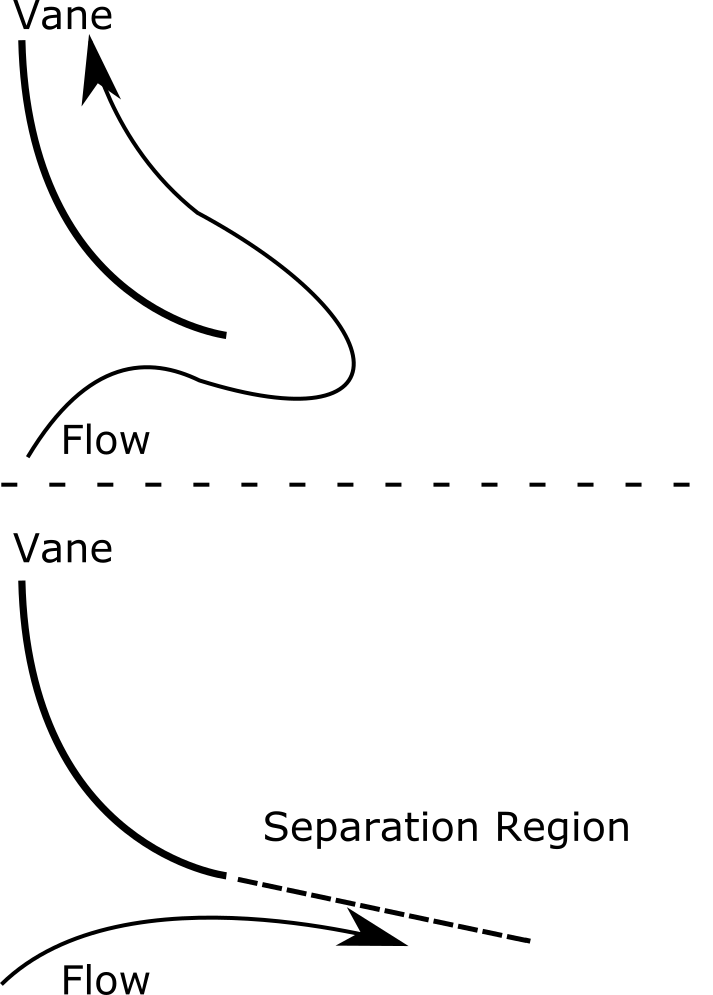
\includegraphics[width = 6 cm]{figs/sep_model}
    \caption{Schematic depicting the separation model that extends past
   the trailing edge of the vanes. In the top case, the flow entering
   the virtual vane region is forced to align with the vane angle despite
   this resulting in a reversal of the flow direction. In the second
   case, the flow continues to move tangent to the vanes due to the
   separation of the boundary layer off the trailing edge.} 
    \label{fig:sep_model}
  \end{center}
\end{figure}

Let $\bf n^v$ be the normal vector to the vanes, and $\bf n^r$ the
normal vector pointing out of the vane region. Then, $\bf t^v$ is the
tangential vector to the vanes pointing out of the vane region and is
defined as
\begin{equation}
 \bf t^v = \left( {\bf n^v_y},{\bf -n_x^v} \right) \text{sign}\left[
	    \left( {\bf n^v_y},{\bf -n_x^v} \right) \cdot {\bf n^r} \right].
\end{equation}\todo{not sure I like this notation}

The forcing is modified when the velocity vector of the local flow, $\bf
u$ is pointing in to the forcing region: ${\bf u} \cdot {\bf n^r} < 0$, and
when the velocity vector is in the same direction as the tangent line to
the vanes: ${\bf u} \cdot {\bf t^v} > 0 $. In these instances, the
forcing acts as if there was a rigid surface past the vane edge, and
gives the appearance of a special ``no-penetration'' condition for the
velocity for these cases.  

The addition of this simple separation model significantly reduced the
flow that penetrated the back of the vanes, and produces results
consistent with the observations provided by our experimental
colleagues.  

\subsection{Effect of Surface Roughness}

%%
%% this does not describe the phenomena being modeled or the precise
%% model -- rewrite
%%
%%
%% this does not say enough about the surface roughness
%% motivate that and explain how it is used, than show your estimate 
%% to argue it is small
%%

Surface roughness effects have been shown to play a role in the
formation of dust-devils and related atmospheric
phenomena\cite{oke1987boundary}. For the flat and sandy regions we are
simulating, the impact is expected to be a small thermal ``kick-up''
versus an entirely smooth surface. This is modeled as a volumetric 
forcing over a narrow height over the surface, 
\begin{equation}
 F^{'''}_{z_0} = \frac{1}{2}\rho V_z^2/z_{0}, 
\end{equation}
and $z_{0}$ is the roughness height. We ensure that the energy
introduced into flow is small fraction of total flow energy by comparing
this with the energy flux through the top of the vanes. The total energy
added is measured as,  
\begin{equation}
 E_{\text{injected}} = \int_0^{2\pi} \int_0^R \int_0^{z_0} F^{'''}_{z_0} dz dr d\theta. 
\end{equation}
R is the outer diameter of the vanes. 
The value of $E_{\text{injected}}$ is typically a few percent of the
total energy kinetic energy flux measured through the top of the
vanes.\todo{surface roughness citation here?}

%This general forcing provides additional capabilities including the
%ability to investigate engineering greater surface roughness or
%structures that could provide greater ``kick-up'' of the thin thermal
%layer near the surface into the flowing regime. It can also support more
%general turning configurations than the virtual vanes outlined above. 
